
\chapter{公式部分参考}\label{chapter2}
\vbox{}\vbox{}

本章第一小节介绍本文使用的一些符号和公式定理;第二小节介绍目前常见的三种张量分解方式,为后文内容准备理论铺垫;第三小节介绍与本文相关的模型,并列举这些模型的优缺点。

\vbox{}
\section{符号及定义}
\vbox{}

在本文中,实数域和复数域分别表示为 $ \mathbb{R} $ 和 $ \mathbb{C} $ 。张量是一种表示多维数据的数学概念,张量阶数为零的数据称作标量,用小写字母表示,如标量 $ a $ ;张量阶数为一的数据称作向量,用加粗的小写字母表示,如向量 $ \mathbf{a}$ ;张量阶数为二的数据称作矩阵,用大写字母表示,如矩阵 $A\in \mathbb{R}^{n_1\times n_2} $ ,用 $ I_n $ 表示 $ n \times n $ 的单位矩阵;对于张量阶数大于等于$ 3 $的数据使用Euler手写字体表示,例如三阶张量 $\mathcal{A} \in \mathbb{R}^{n_1\times n_2\times n_3}$ ,用 $ \mathcal{I}_n $ 表示 $ n \times n \times n $的单位张量。图\ref{figure_tensor}表示不同阶数张量的示意图,一个立方体表示一个元素。本文主要对三阶张量进行研究。


\begin{figure}[htbp]
	\centering
	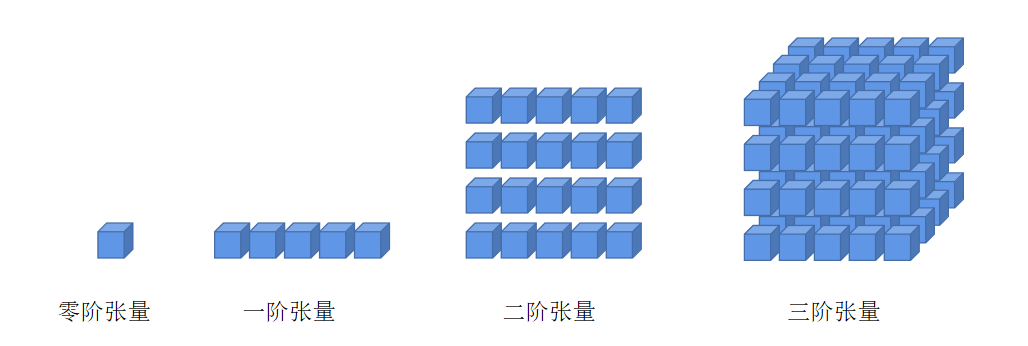
\includegraphics[scale=0.5]{pic/chap2/1.png}
	\bicaption{张量示意图}	
	{Tensor diagram.}
	\label{figure_tensor}
\end{figure}

向量 $ \mathbf{a} $ 中的第$ i $个元素记作 $ a_i $;矩阵$ A $中的第 $ (i,j) $ 个元素记作 $ A_{i,j} $ ;三阶张量 $ \mathcal{A} $ 中的第 $ (i,j,k) $ 个元素记作 $ \mathcal{A}_{i,j,k} $ 。在矩阵中使用行和列表示其子序列,分别表示矩阵在某一行或某一列中的所有元素,本文中使用冒号表示某行(列)的所有元素,如矩阵 $ A $ 的第 $ j $ 列元素表示为 $ A_{:,j} $ ,$ A $ 的第$ i $行表示为$ A_{i,:} $。

在三阶张量中,一共有三个维度,通常使用张量纤维(fiber)表示不同维度下的元素向量。除了行 $ \mathcal{A}_{:,j,k} $ 和列 $ \mathcal{A}_{i,:,k} $ 外,三阶张量中引入了管道(tube)表示第三维度中的子元素向量 $ \mathcal{A}_{i,j,:} $ 。图\ref{figure_fiber}表示三种不同的张量纤维。从张量中提取出来的纤维一般是以列向量的方式表示。

\begin{figure}[htbp]
	\centering
	\subfigure[列纤维:$ \mathcal{A}_{:,j,k} $]{
		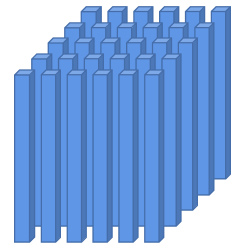
\includegraphics[width=1.7in]{pic/chap2/2_1.png}} 
	\subfigure[行纤维:$ \mathcal{A}_{i,:,k} $]{
		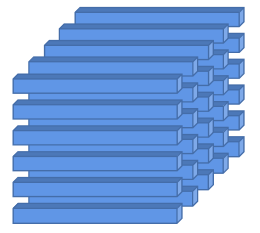
\includegraphics[width=1.9in]{pic/chap2/2_2.png}}
	\subfigure[管纤维:$ \mathcal{A}_{i,j,:} $]{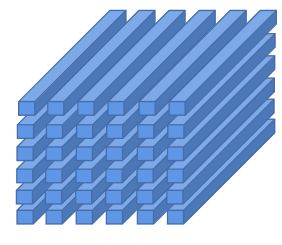
\includegraphics[width=1.9in]{pic/chap2/2_3.png}}
	\bicaption{三种张量纤维}	
	{Three kind of tensor fibers.}
	\label{figure_fiber}
\end{figure}

张量切片(slice)表示张量的二维截面(矩阵形式),是由一个固定维度中的索引构成的。以三阶张量为例,根据固定维度的不同,可以得到张量的水平切片 $ \mathcal{A}_{i,:,:} $ ,侧面切片 $ \mathcal{A}_{:,j,:} $ 和前置切片 $ \mathcal{A}_{:,:,k} $ ,图\ref{figure_slice}表示三种模态的张量切片的视觉效果图,从张量中提取出来的切片是矩阵的形式。

\begin{figure}[htbp]
	\centering
		\subfigure[水平切片:$ \mathcal{A}_{i,:,:} $]{
		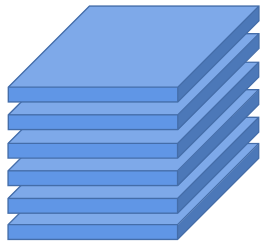
\includegraphics[width=1.9in]{pic/chap2/3_1.png}} 
	\subfigure[侧面切片:$ \mathcal{A}_{:,j,:} $]{
		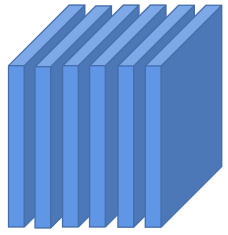
\includegraphics[width=1.8in]{pic/chap2/3_2.png}}
	\subfigure[前置切片:$ \mathcal{A}_{:,:,k} $ ]{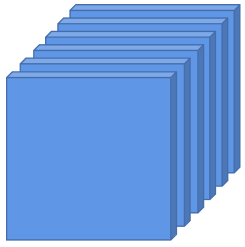
\includegraphics[width=1.9in]{pic/chap2/3_3.png}}
	\bicaption{三种张量切片}	
	{Three kind of tensor slices.}
	\label{figure_slice}
\end{figure}

矩阵 $ A $ 和 $ B $ 之间的内积定义为 $ \left<A,B\right> = Tr(A^*B) $ ,其中 $ A^* $ 表示矩阵$ A $ 的共轭转置,$ Tr() $ 表示矩阵的迹函数。张量 $ \mathcal{A} $ 和 $ \mathcal{B} $ 在 $  \mathbb{C}^{n_1\times n_2\times n_3} $ 的内积定义为 $ \left< \mathcal{A} , \mathcal{B} \right> = \sum_{i=1}^{n_3} \left<\mathcal{A}_{:,:,i},\mathcal{B}_{:,:,i} \right> $。

向量和矩阵分别有三种范数,对于向量 $ \mathbf{v}\in \mathbb{R}^n $,其三种范数分别为:(1)$ L_0 $范数 $ \left|\left| \mathbf{v} \right|\right|_0= \# \left\{i,\mathbf{v}_i \ne 0 \right\} $ ;(2) $ L_1 $ 范数 $ \left|\left| \mathbf{v} \right|\right|_1= \sum_i \left| \mathbf{v}_i \right|$;(3) $ L_2 $ 范数 $ \left|\left| \mathbf{v} \right|\right|_2= \sqrt{\sum_i \left| \mathbf{v}_i \right|} $。对于矩阵 $ A\in\mathbb{R}^{n_1\times n_2} $,其三种范数分别为:(1)谱范数 $ \left|\left| A \right|\right|=\max_i\sigma_i(M)$ ,其中 $ \sigma(A) $ 为奇异值向量;(2)核范数 $ \left|\left| A \right|\right|_*= \sum_i \sigma_i(M) $;(3)Frobenius范数 $ \left|\left| A \right|\right|_F = \sqrt{\sum_{ij}\left|M_{i,j}\right|^2} $。对于张量 $ \mathcal{T} \in \mathbb{R}^{n_1 \times n_2 \times n_3 } $ ,其范数分别定义为:(1)$ L_1 $ 范数 $ \left|\left| \mathcal{T} \right|\right|_1= \sum_{ijk} \left| \mathcal{T}_{i,j,k} \right|$ ;(2)Frobenius范数 $ \left|\left| \mathcal{T} \right|\right|_F = \sqrt{\sum_{ijk}\left|\mathcal{T}_{i,j,k}\right|^2} $;(3)无穷范数 $ \left|\left| \mathcal{T} \right|\right|_{\infty} = \max_{i,j,k}\left|\mathcal{T}_{i,j,k}\right| $。

以上是本文主要使用的符号意义。为了易读性,本文将常用符号用表格整理,详情见表\ref{tab:notation}。对于上文和表格中未给出的符号,本文会在该符号第一次出现的位置给予说明。

\begin{table}[]
	\centering
	\bicaption{公式}
	{notation.}
	\label{tab:notation}
	\begin{tabular}{c c|c c}
		\toprule
		公式                                          & 解释                                                                                                                       & 公式                                      & 解释                                                      \\ \midrule[0.5pt]
		$\mathbb{R}$                                       & 实数域                                                                   &                    	$ \mathbb{C}  $                                    & 复数域         \\       
		     $ a $    &  标量  &	         $  \textbf{a} $                                    & 向量            \\  
		$A $                                     & 矩阵                 &       $ \mathcal{A} $                                & 张量 	                                 \\ 
		$\textbf{A} $                                   & 集合   &	$ \textbf{a}_i $                                   & $  \textbf{a} $ 中的第 $ i $ 个元素  \\ 
		$ \textbf{0}_{m\times n} $                         & $m\times n $ 空矩阵                                &          		$ A_{i,j} $                                        & $A$ 中的第($ i,j $)个元素                          \\    
		$ \sigma_i( A ) $                          & 
		矩阵 $ A $ 中的第 $ i $ 个奇异值	   &                             	$ \sigma(A) $                             & $ (\sigma_1( A ),\sigma_2( A ),\dots,\sigma_r( A )^T$                            \\  
		$ A^* $                                   & $ A $ 的共轭转置   &	$ \operatorname{Conj}(A) $                         & $A$ 的共轭        \\  
		
		$\mathcal{A}_{i, j, k}$                        & $ \mathcal{A}$ 的第 $ (i,j,k) $ 个元素                                                                 & $ \mathcal{A}_{i,j,:} $                        & $ \mathcal{A}$ 的第 $ (i,j) $ 个管道                                                 \\  
		
		
		$ \mathcal{A}_{:,:,i} $     & $ \mathcal{A}$ 的第 $ i $ 个前置切片   &     $\mathcal{A}^{\dag} $                         & $ \mathcal{A} $ 的伪逆                                            \\  
		$ \mathcal{\bar A} $                           &  $ \mathrm{fft}(\mathcal{A},[],3) $                                                &        $\bar A$                      &     $ \mathrm{bdiag}(\mathcal{\bar A})$           \\  
		$ \mathrm{\bar A}_{i} $                        & $ \mathcal{\bar A} $ 的第 $ i $ 个前置切片         	&                           $\#\textbf{A}$  	&$ \textbf{A} $ 中的元素个数                   \\ \bottomrule
	\end{tabular}
\end{table}



\begin{figure}[htbp]
	\centering
	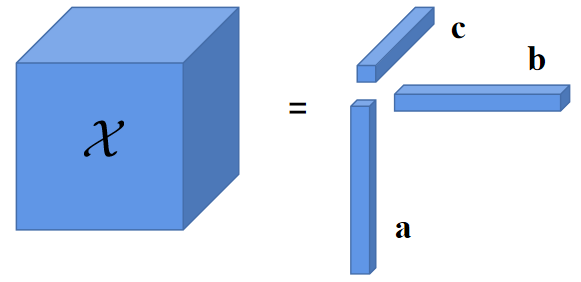
\includegraphics[scale=0.5]{pic/chap2/4.png}
	\bicaption{三阶秩一张量}	
	{Rank-one thrid-order tensor.}
	\label{figure_rankone}
\end{figure}



\vbox{}
\section{张量分解}
\vbox{}

1927年,Hitchcock\cite{hitchcock1927expression}提出了张量分解的概念,通过有限个秩一张量的多线性乘积表示完整的张量,可以大大降低高阶张量的数据量,提高了计算效率。由于张量分解可以将高阶张量中的有效信息提取出来,因此张量分解被广泛的应用于大数据分析\cite{song_tensor_2019,sael_scalable_2015},图象处理\cite{zhou_tensor_2017,song_nonlocal_2018}等各个领域,下面介绍一些常见的张量分解模型。

\subsection{CP分解}

\begin{definition}
	(秩一张量) 如果一个N阶张量$ \mathcal{A}\in \mathbb{R}^{n_1\times n_2\times \cdots \times n_N} $可以写做由$ N $个向量的外积的构成,如$ \mathcal{A}=\mathbf{a}^{(1)}\circ \mathbf{a}^{(2)} \circ \cdots \circ \mathbf{a}^{(N)} $,其中符号$ \circ $表示向量外积,$ \mathbf{a}^{(i)} $表示张量中第$ i $个模态的向量。也就意味着张量中的每个元素都可以表示为不同模式的向量元素的乘积,如$ \mathcal{A}_{i_1i_2\cdots i_N}=a^{(1)}_{i_1}a^{(2)}_{i_2}\cdots a^{(N)}_{i_N}  $。图\ref{figure_rankone}展示了一种三阶的秩一张量。
\end{definition}

张量CP分解是CANDECOMP/PARAFAC分解\cite{kolda_tensor_2009}的简称。CP分解于上个世纪70年代被提出\cite{carroll_analysis_1970,harshman1970foundations},一直受到广大学者的青睐与研究,以此为基础的张量恢复方法层出不穷。张量CP分解是将一个张量分解为一组秩一张量相加的形式。比如说,给定一个三阶张量 $ \mathcal{A}\in \mathbb{R}^{n_1\times n_2\times n_3} $ ,本文将其写为 $ \mathcal{A}\approx  \sum_{r=1}^{R}\mathbf{a}_r\circ \mathbf{b}_r \circ  \mathbf{c}_r$ 的形式,其中$ R $是一个正整数,$ \mathbf{a}_r\mathbf{b}_r\mathbf{c}_r $ 分别为三阶张量不同模态下的向量,$ r=1,\cdots,R $。为了更加生动形象的表示出CP分解模型,图\ref{figure_cp}中展示了三阶张量的CP分解模型。
\begin{figure}[htbp]
	\centering
	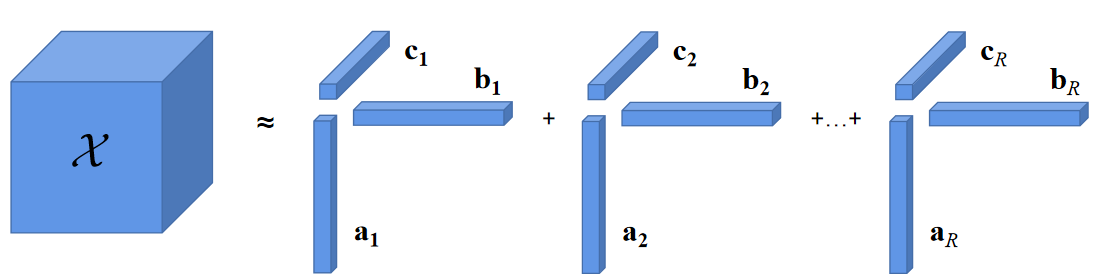
\includegraphics[scale=0.5]{pic/chap2/5.png}
	\bicaption{三阶张量的CP分解}	
	{CP decomposition of a three-way array.}
	\label{figure_cp}
\end{figure}

张量CP分解的效果取决于$ R $的大小,一个合适的$ R $可以更加准确的表示一个张量。目前,没有一个准确的算法可以确定$ R $的大小,故计算张量的CP分解中的$ R $值还是一个NP难问题。在实践中,一般需要通过多次实验比较找出一个最优的$ R $值,这样会耗费大量的计算资源。

\subsection{Tucker分解}
Tucker分解是由Tucker\cite{tucker1966some}在1963年提出的,并得到了学术界的广泛使用。Tucker分解是一种高阶的主成分分析,它将张量分解成了由一个核心张量和张量在不同模式展开的矩阵相乘的形式。对于一个三阶张量 $ \mathcal{A}\in \mathbb{R}^{n_1\times n_2\times n_3} $ ,它的Tucker分解的形式可以写作:$ \mathcal{A}\approx \mathcal{G}\times_1A^{(1)}\times_2A^{(2)}\times_3A^{(3)} $,其中$ A^{(1)}A^{(2)}A^{(3)} $分别表示张量$ \mathcal{A} $在不同模态下展开的矩阵。为方便理解Tucker分解,请看图\ref{figure_tucker}。Tucker分解的秩可以用一下数学公式表示:
\begin{equation}
\text{rank}_{\text{Tucker}}(\mathcal{A})=[R_1,R_2,\cdots,R_K]^T	
\end{equation}
其中$ R_K $表示张量$ \mathcal{A} $在第$ K $模态下展开的矩阵的秩的大小,将张量每个模态矩阵的秩结合起来就是Tucker分解的秩。

尽管Tucker分解有着较好的表征能力,但是分解得到的核心张量$ \mathcal{G} $会随着张量阶数的增长成指数型增长,容易产生数据维度灾难的问题,限制了其在高阶数据中的应用。

\begin{figure}[htbp]
	\centering
	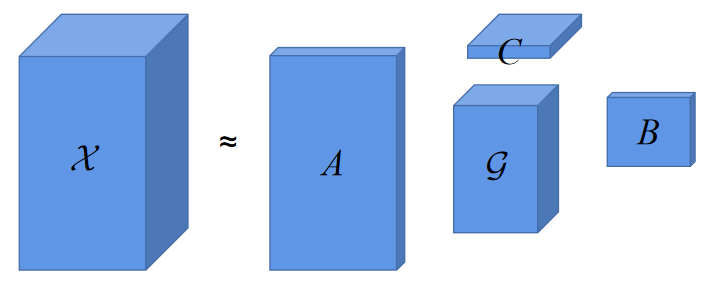
\includegraphics[scale=0.5]{pic/chap2/6.png}
	\bicaption{三阶张量的Tucker分解}	
	{Tucker decomposition of a three-way array.}
	\label{figure_tucker}
\end{figure}

\subsection{张量奇异值分解}
张量奇异值分解模型是由Kilmer等人\cite{18}于2011年提出,Kilmer等人首先提出了一些新的张量的运算方式(如张量乘积),基于这些张量运算,提出了张量奇异值分解,该分解方法是将张量转化打傅里叶变换域,再对张量中的每一个前置切片进行矩阵奇异值分解操作,在变换域中得到最优的低秩近似结构。图\ref{figure:tsvd}展示了三阶张量t-SVD的示意图。下面介绍t-SVD的基础概念。

对张量进行张量奇异值分解需要先将张量做离散傅里叶变换(DFT),将张量中的数据从实数域变换到傅里叶域,具体操作见文献\cite{18}。本文将DFT后的张量$ \mathcal{A} $用$  \bar{\mathcal{A}}  $表示。在MATLAB中,通常使用$ \mathrm{fft} $命令对数据做DFT处理,比如对于三阶张量$ \mathcal{A} $:$ 	\mathcal{\bar A}=\mathrm{fft}(\mathcal{A},[], 3)$。使用$ \mathrm{ifft} $命令将 $ \bar{\mathcal{A}} $ 逆变换回 $ \mathcal{A} $,如:$ \mathcal{A}=\mathrm{ifft}(\bar{\mathcal{A}},[], 3) $。

\begin{figure}[htbp]
	\centering
	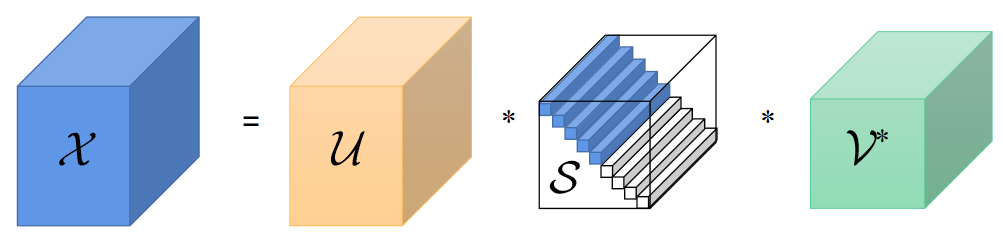
\includegraphics[scale=0.5]{pic/chap2/7.png}
	\bicaption{张量奇异值分解}	
	{Tensor SVD decomposition.}
	\label{figure:tsvd}
\end{figure}

\begin{definition}\label{def:tprod}
(张量乘积\cite{18})设$\mathcal{A}\in \mathbb{R}^{n_1\times n_2 \times n_3}$和$\mathcal{B}\in \mathbb{R}^{n_2\times l \times n_3 }$,$ \mathcal{A} $和$ \mathcal{B} $经过张量乘积后的结果是一个尺寸为$n_1\times l \times n_3$的张量,公式为:
	\begin{equation}
		\mathcal{A}\ast\mathcal{B}=\mathrm{fold}(\mathrm{bcirc}(\mathcal{A})\cdot \mathrm{unfold}(\mathcal{B}))
	\end{equation}
其中$\cdot$表示矩阵乘法,$	\mathrm{unfold}(\cdot)$表示将张量展开为矩阵,例如 $ \mathcal{B}\in \mathbb{R}^{n_1\times n_2\times n_3} $ :\begin{equation}
\mathrm{unfold}(\mathcal{B})=\left(
\begin{array}{c}
	\mathcal{B}_{:,:,1} \\
	\mathcal{B}_{:,:,2} \\
	\vdots \\
	\mathcal{B}_{:,:,n_3} \\
\end{array}
\right)\in \mathbb{R}^{n_1n_3  \times n_2},  \end{equation} $\mathrm{fold}(\cdot)$是$	\mathrm{unfold}(\cdot)$的逆运算,表示将矩阵折叠为张量:$\mathrm{fold}(\mathrm{unfold}(\mathcal{B}))=\mathcal{B}$。
\end{definition}

\begin{definition}
(块循环矩阵\cite{18})张量$\mathcal{A}\in \mathbb{R}^{n_1\times n_2 \times n_3}$的块循环矩阵表示为$ \mathrm{bcirc} (\mathcal{A}) \in \mathbb{R}^{n_1n_3\times n_2n_3}$,具体表示为:\begin{equation}\mathrm{bcirc}(\mathcal{A})=\left(
\begin{array}{cccc}
	\mathcal{A}_{:,:,1}& \mathcal{A}_{:,:,n_3}  & \cdots & \mathcal{A}_{:,:,2}  \\
	\mathcal{A}_{:,:,2} &  \mathcal{A}_{:,:,1}  & \cdots&  \mathcal{A}_{:,:,3} \\
	\vdots  & \vdots & \ddots & \vdots \\
	\mathcal{A}_{:,:,n_3}  & \mathcal{A}_{:,:,n_3-1}   & \cdots &  	 \mathcal{A}_{:,:,1}  \\
\end{array}                               \right).	\end{equation}
\end{definition}

\begin{algorithm}[!htbp]
	\caption{张量奇异值分解\cite{34}}\label{alg:tsvd}
	\begin{algorithmic}[1]
		\State \textbf{输入:}$\mathcal{Y}\in \mathbb{R}^{n_1 \times n_2 \times n_3}$, $\lambda>0$
		\State \textbf{输出:}$\mathcal{U}$, $\mathcal{S}$ and $ \mathcal{V}$
		\State 计算$\mathcal{\bar Y} =\mathrm{fft}(\mathcal{Y} ,[],3)$;
		\State 通过下式计算从$\mathcal{\bar Y} $分解得到的$\mathcal{\bar U} $,$\mathcal{\bar S} $和$\mathcal{\bar V} $的每个前置切片;
		\For{$i=1,...,\lfloor\frac{n_3+1}{2}\rfloor$}
		\State$[\bar U^{(i)},\bar S^{(i)}, \bar V^{(i)}]=\text{SVD}(\bar Y^{(i)})$;
		\EndFor
		\For{$i=\lfloor\frac{n_3+1}{2}\rfloor+1,\cdots,n_3$}
		\State$\bar U^{(i)}=Conj(\bar U^{(n_3-i+2)})$;
		\State$\bar S^{(i)}= \bar S^{(n_3-i+2)}$;
		\State$\bar V^{(i)}=Conj(\bar V^{(n_3-i+2)})$;
		\EndFor
		\State$\mathcal{U}=\mathrm{ifft}(\bar U ,[],3)$, $\mathcal{S}=\mathrm{ifft}(\bar S,[],3)$ and $ \mathcal{V}=\mathrm{ifft}(\bar V,[],3)$。
	\end{algorithmic}
\end{algorithm}

\begin{definition}
	(全对角张量\cite{18})如果张量$ \mathcal{A} $的每个前置切片都为对角矩阵,就称该张量为全对角张量。
\end{definition}

\begin{definition}
	(单位张量\cite{18})如果张量$\mathcal{I}_{n \times n  \times n_3} \in \mathbb{R}^{n \times n  \times n_3}$的第一层前置切片为单位矩阵,其余前置切片全为0矩阵,就称该张量为单位张量。
\end{definition}

\begin{definition}
	(共轭转置\cite{18})张量$\mathcal{A}\in \mathbb{C}^{n_1\times n_2 \times n_3}$的共轭转置表示为$\mathcal{A}^*\in \mathbb{C}^{ n_2 \times n_1  \times n_3} $。是将张量的每个前置切片做共轭转置,然后将转置后的前置切片的顺序从位置2反转到位置3。
\end{definition}

\begin{definition}
	(正交张量\cite{18})如果张量$\mathcal{Q}\in \mathbb{C}^{n\times n \times n_3}$满足$\mathcal{Q}^* \ast  \mathcal{Q}=\mathcal{Q} \ast \mathcal{Q}^*=\mathcal{I}_{n\times n \times n_3}$,则该张量为正交张量。
\end{definition}

\begin{theorem}
	(张量奇异值分解\cite{18})设张量$\mathcal{A}\in \mathbb{R}^{n_1\times n_2 \times n_3}$,它可以被因式分解为	
	\begin{equation}\label{equ:svd}
	\mathcal{A}=\mathcal{U} \ast \mathcal{S} \ast \mathcal{V}^*	,
	\end{equation}
	其中$\mathcal{U}  \in \mathbb{R}^{n_1\times n_1 \times n_3 }$和$\mathcal{V} \in \mathbb{R}^{n_2\times n_2 \times n_3 }$为正交张量,$\mathcal{S} \in\mathbb{R}^{n_1\times n_2 \times n_3}$为全对角张量。分解\ref{equ:svd}就叫做张量奇异值分解,更多细节见算法\ref{alg:tsvd}
\end{theorem}

\begin{definition}
	(张量管秩\cite{18})对于张量$\mathcal{A}\in \mathbb{R}^{n_1\times n_2 \times n_3}$,他的张量管秩表示为$\mathrm{rank}_\mathrm{t}(\mathcal{A})$,其定义为$\mathcal{S}$非零奇异管的的个数,这里的$\mathcal{S}$为经过张量奇异值分解得到的$
	\mathcal{A}=\mathcal{U} \ast \mathcal{S} \ast \mathcal{V}^*	$。张量管秩可以用数学公式表达:$\mathrm{rank}(\mathcal{A})=\#\{i|\mathcal{S}(i,i,:)\neq \textbf{0}\}=\#\{i|\mathcal{S}(i,i,1)\neq  0\}$。 
\end{definition}

\begin{definition}
	(张量核范数 \cite{34})对于张量$\mathcal{A}\in \mathbb{R}^{n_1\times n_2 \times n_3}$,他的张量奇异值分解表示为 $\mathcal{A}=\mathcal{U} \ast \mathcal{S} \ast \mathcal{V}^*$,其张量核范数记作$ \|\mathcal{X}\|_{*} $,定义为 $\|\mathcal{X}\|_*=\sum_{i=1}^{\mathrm{rank}_t(\mathcal{X})}\mathcal{S}_{i,i,1}$。 
\end{definition}





